         \chapter{Fisiese en chemiese verandering}\fancyfoot[LO,RE]{Chemistry: Chemical change}
    \setcounter{figure}{1}
    \setcounter{subfigure}{1}
    \label{m38709*cid1}
            \section{Inleiding}
            \nopagebreak


      \label{m38709*id62175}Materie is oral rondom ons. Die lessenaars waarby ons sit, die lug wat ons inasem en die water wat ons drink, is almal
voorbeelde van materie. Materie bly egter nie altyd dieselfde nie. Dit kan op baie verskillende
maniere verander. In hierdie hoofstuk gaan ons die \textbf{fisiese} en \textbf{chemiese} veranderings wat materie ondergaan, van naderby
beskou.\par 
    \label{m38709*cid2}
            \subsection*{Fisiese veranderings in materie}
            \nopagebreak
      \label{m38709*id62200}'n \textbf{Fisiese verandering}is een waar die deeltjies van die stowwe wat betrokke is in die verandering
nie op enige wyse afgebreek word nie. Byvoorbeeld wanneer water verhit word, neem die temperatuur en energie van
die watermolekules toe en die vloeibare water verdamp om waterdamp te vorm.Wanneer dit gebeur, vind daar ‘n soort
verandering plaas, maar die molekulêre struktuur van die water verander nie. Dit is 'n voorbeeld van 'n \textsl{fisiese verandering}. Alle veranderings in toestand is fiesiese veranderings. \par 
      \label{m38709*id62556}$\text{H}{}_{2}\text{O}\left( \ell \right)\to \text{H}{}_{2}\text{O}\left(\text{g}\right)$
      \par 
      \label{m38709*id62600}Geleiding (die oordrag van energie deur 'n materiaal) is nog 'n voorbeeld van 'n fisiese verandering. Soos \textsl{energie} oorgedra word van een materiaal na 'n ander, word die \textsl{energie} van elke materiaal verander, maar sy chemiese samestelling bly onveranderd. Die oplossing van een stof in 'n ander een, is ook 'n fisiese verandering.\par 
\label{m38709*fhsst!!!underscore!!!id76}
 \Definition{   \label{id2458225}Fisiese verandering } { \label{m38709*meaningfhsst!!!underscore!!!id76}
      'n Verandering wat gesien of gevoel kan word, maar wat nie gepaard gaan met die afbreek van partikels tydens die
reaksie nie. Tydens 'n fisiese verandering, kan die \textsl{vorm} van materie verander, maar nie sy \textsl{identiteit} nie. 
       } 

      \label{m38709*id62640}Daar is 'n paar belangrike dinge om te onthou rakende die fisiese veranderings in materie:\par 
      \label{m38709*id62644}\begin{enumerate}[noitemsep, label=\textbf{\arabic*}. ] 
            \label{m38709*uid1}\item \textsl{Rangskikking van deeltjies}\newline
Wanneer 'n fisiese verandering plaasvind, kan die verbindings hulself her-rangskik, maar die
bindings tussen die atome sal nie breek nie. Byvoorbeeld wanneer vloeibare water kook, sal molekules uitmekaar
beweeg, maar die molekules sal ongeskonde bly. Met ander woorde, water sal nie opbreek in waterstof- en suurstof atome
nie.

Figuur~\ref{fig:physical change:water phases} toon hierdie fase-verandering. Let daarop dat die watermolekules onveranderd bly, terwyl die rangskikking van die molekules wel verander.
    \setcounter{subfigure}{0}
	\begin{figure}[H] % horizontal\label{m38709*uid2}
\begin{figure}[h]
\begin{center}
\begin{pspicture}(0,0)(10,2.6)
\SpecialCoor
%\psgrid[gridcolor=lightgray]
\def\water{\psset{unit=0.25}\rput{150}{\pscircle(0,0){2}
\psarc[fillcolor=white,fillstyle=solid](-1.5,1){1.5}{30}{260}
\psarc[fillcolor=white,fillstyle=solid](1.5,1){1.5}{280}{150}
\rput(-1.5,1){\pscurve(1.5;30)(-1;142.5)(1.5;260)}
\rput(1.5,1){\pscurve(1.5;150)(-1;37.5)(1.5;280)}}}

\rput(2,0){\psframe(0,0.5)(3,2.5)
\rput(1.5,1){\psset{unit=0.5}\rput(-0.7,-0.2){\water}
\rput{185}(-1,0.9){\water}
\rput{120}(2,0.6){\water}
\rput{310}(-2.1,0){\water}
\rput{60}(0.6,1.1){\water}
\rput(1.2,-0.2){\water}}}

\rput(5,0){\psframe(0,0.5)(3,2.5)
\rput(1.5,1){\psset{unit=0.5}\rput{120}(2,1){\water}
\rput{250}(-1,2){\water}
\rput{70}(0,.5){\water}
\rput{150}(-1.5,-.2){\water}}}

\uput[d](3,0.5){vloeistof}
\uput[d](6,0.5){gas}

\end{pspicture}
\end{center}
\caption{Die rangskikking van water molekules in die vloeistof- en gasfase}
\label{fig:physical change:water phases}
\end{figure}
 \end{figure}   
\IFact{Die binding van waterstof en suurstof om water te vorm, is ‘n baie hewige reaksie en as die watermolekules
uitmekaar sou breek elke keer as water gekook word, sou lewe op aarde nie vir baie lank bly bestaan het nie!}    
\label{m38709*uid221}\item \textsl{Die behoud van massa}\newline In 'n fisiese verandering, sal die totale massa, die aantal atome en die aantal molekules altyd dieselfde bly. Met ander woorde, jy sal altyd dieselfde aantal molekules
of atome aan die einde van die verandering kry as wat jy aan die begin gehad het.
\label{m38709*uid3}\item \textsl{Energie-veranderings}\newline
Energie-veranderinge kan plaasvind tydens 'n fisiese verandering in materie, maar hierdie
energie-veranderinge is normaalweg kleiner as die energie-veranderinge wat plaasvind tydens 'n
chemiese verandering.
\label{m38709*uid4}\item \textsl{Omkeerbaarheid}\newline
Fisiese veranderings in materie is gewoonlik makliker omkeerbaar as chemiese veranderings. Metodes
soos filtrasie en distillasie kan gebruik word om veranderings om te keer. Verandering in tem-
peratuur is 'n ander manier om' n fisiese verandering om te keer. Byvoorbeeld, 'n mengsel van sout en
water kan deur filtrasie geskei word, terwyl ys verander kan word na vloeibare water en andersom deur verandering van
die temperatuur.
\end{enumerate}
        \label{m38709*eip-904}\begin{activity}{Fisiese verandering}Gebruik plastiek korrels of albasters om water in di vaste toestand te verteenwoordig. Wat moet jy doen met die korrels om die verandering van 'n vastestof na 'n vloeistof voor te stel?\\
Maak 'n mengsel van sand en water. Filteer hierdie mengsel. Wat neem jy waar? \\
Maak 'n mengsel van ystervylsels en swael. Kan jy die mengsel met 'n magneet skei?
\end{activity}
\pagebreak
\label{m38709*secfhsst!!!underscore!!!id243}
            \begin{g_experiment}{Chemiese reaksie tussen yster en swael}
            \nopagebreak
            \label{m38709*id63437}\noindent{}\textbf{Doel:}
          \newline
     Demonstrasie van die reaksie tussen yster en swael om ystersulfied te vorm.\par 
        \label{m38709*id63447}\noindent{}\textbf{Apparaat:}
          \newline
$5,6~\text{g}$ ystervylsels en $3,2~\text{g}$ verpoeierde swael; porselein bakkie; proefbuis; Bunsenbrander\par 
        \label{m38709*id63457}
    \setcounter{subfigure}{0}
	\begin{figure}[H] % horizontal\label{m38709*id63460}
    \begin{center}
\begin{pspicture}(0,0)(5,5)
\psset{unit=0.5cm,tubeSeul=true,pince=true}
\newpsstyle{gray} {linestyle=none,fillstyle=solid,fillcolor=darkgray}
\newpsstyle{orange} {linestyle=none,fillstyle=solid,fillcolor=orange}
%playing with colours, try tweak this to look like the real thing, add photo of the real thing?
\pstChauffageTube[aspectLiquide1=gray,aspectLiquide2=orange,niveauLiquide1=40,niveauLiquide2=20]
\end{pspicture}
    \end{center}
 \end{figure}       
        \par 
        \label{m38709*id63467}\noindent{}\textbf{Metode:}
          \newline
        \label{m38709*id63473}\begin{enumerate}[noitemsep, label=\textbf{\arabic*}. ] 
            \label{m38709*uid20}\item Weeg die hoeveelheid yster en swael wat jy benodig sorgvuldig en meng dit in 'n porselein bakkie.
\label{m38709*uid21}\item Neem 'n klein hoeveelheid van hierdie mengsel en plaas dit in die proefbuis. Die proefbuismoet ongeveer een derde vol wees.
\label{m38709*uid22}\item Hierdie reaksie moet plaasvind in 'n dampkas of binne 'n goed geventileerde kamer. Verhit die proefbuis met die mengsel oor ‘n Bunsenbrander. Verhoog die hitte indien geen reaksie plaasvind nie. Sodra die reaksie begin, moet jy die proefbuis uit die vlam verwyder. Skryf jou waarnemings neer.
\label{m38709*uid23}\item Wag vir die produk om af te koel voordat jy ‘n hamer gebruik om die proefbuis te breek. Maak seker dat die proefbuis in papier toegedraai is voordat jy dit breek om beserings te voorkom.
\label{m38709*uid24}\item Hoe lyk die produk? Lyk dit soos die oorspronklike reaktanse? Beskik dit nog oor enige van die eienskappe van
die reaktanse? (bv die magnetisme van yster)?
\end{enumerate}
        \par 
        \label{m38709*eip-963}
      \Warning{Wanneer jy ‘n Bunsenbrander gebruik, sorg dat jy binne ‘n goed geventileerde ruimte werk en maak seker dat daar
geen vlambare stowwe in die nabyheid is nie. Steek loshangende kledingstukke in en maak lang hare vas!}
	\par
      \label{m38709*id63554}\noindent{}\textbf{Resultaat:}
          \newline
        \label{m38709*id63560}\begin{enumerate}[noitemsep, label=\textbf{\arabic*}. ] 
            \label{m38709*uid25}\item Nadat jy die proefbuis uit die vlam verwyder het, sal die mengsel gloei met 'n helderrooi kleur. Die reaksie is
eksotermies en \textsl{stel hitte} vry.
\label{m38709*uid26}\item Die produk, ystersulfied, is donker van kleur en vertoon geen van die eienskappe van die oorspronklike reagense nie. Dit is 'n totaal nuwe produk.
\end{enumerate}
        \par 
        \label{m38709*id63594}\noindent{}\textbf{Gevolgtrekkings:}
          \newline
'n Sintersereaksie het plaasgevind. Die vergelyking vir die reaksie is as volg:
        \label{m38709*id63604}\nopagebreak\noindent{}
    \begin{equation*}
    \text{Fe (s)}+\text{S (s)}\to \text{FeS (s)}
      \end{equation*}
    \par 
\end{g_experiment}
    \label{m38709*cid3}
            \subsection*{Chemiese veranderings in materie}
            \nopagebreak
      \label{m38709*id62778}Wanneer 'n \textbf{chemiese verandering} plaasvind, word nuwe stowwe gevorm tydens 'n chemiese reaksie. Hierdie nuwe produkte kan eienskappe vertoon wat baie verskil van die eienskappe van die oorspronklike stowwe aan die begin van die reaksie.\par 
            
\mindsetvid{Chemical change}{VPbfo}

 \Definition{Chemiese verandering} { \label{m38709*meaningfhsst!!!underscore!!!id107}
     Die vorming van nuwe stowwe tydens 'n chemiese reaksie. Een vorm van materie word heeltemaal verander na iets nuuts.
       } 
Ons sal kyk na twee voorbeelde van chemiese verandering: die ontbinding (afbreek) van waterstofperoksied en die sintese
(vorming) van water. \\
\subsubsection*{Ontbinding van waterstofperoksied}
      \label{m38709*id62788}Die ontbinding (afbreek) van waterstofperoksied ($\text{H}_{2}\text{O}_{2}$) om water ($\text{H}_{2}\text{O}$) en suurstofgas ($\text{O}_{2}$) is 'n voorbeeld van 'n chemiese verandering. 'n Vereenvoudige diagram van hierdie reaksie word in  Figuur~\ref{fig:chemical change:decomposition} voorgestel. Die chemiese bindings tussen $\text{O}$ en $\text{H}$ in $\text{H}_{2}\text{O}_{2}$ word gebreek en nuwe bindings tussen $\text{H}$ en $\text{O}$ (om $\text{H}_{2}\text{O}$ te vorm) en tussen $\text{O}$ en $\text{O}$ (om $\text{O}_{2}$ te vorm) word gevorm. 'n Chemiese verandering het plaasgevind.\par 
    \setcounter{subfigure}{0}
\begin{figure}[H]
\begin{center}
\scalebox{.8}{
\begin{pspicture}(-6,-1.5)(12,1.5)
%\psgrid[gridcolor=lightgray]
%reactants
\rput(-2,0){
\psellipse(-3,0)(0.5,0.5)
\rput(-3,0){$\text{O}$}
\psellipse(-2,0)(0.5,0.5)
\rput(-2,0){$\text{O}$}
\psellipse(-3.3,-0.75)(0.3,0.3)
\rput(-3.3,-0.75){$\text{H}$}
\psellipse(-1.7,0.75)(0.3,0.3)
\rput(-1.7,0.75){$\text{H}$}
\rput(3,0){
\psellipse(-3,0)(0.5,0.5)
\rput(-3,0){$\text{O}$}
\psellipse(-2,0)(0.5,0.5)
\rput(-2,0){$\text{O}$}
\psellipse(-3.3,-0.75)(0.3,0.3)
\rput(-3.3,-0.75){$\text{H}$}
\psellipse(-1.7,0.75)(0.3,0.3)
\rput(-1.7,0.75){$\text{H}$}
}
%products
\psline[arrows=->](2,0)(4,0)
\psellipse(5,0)(0.5,0.5)
\rput(5,0){$\text{O}$}
\psellipse(4.5,0.65)(0.3,0.3)
\rput(4.5,0.65){$\text{H}$}
\psellipse(5.5,0.65)(0.3,0.3)
\rput(5.5,0.65){$\text{H}$}
\rput(2,-0.5){
\psellipse(5,0)(0.5,0.5)
\rput(5,0){$\text{O}$}
\psellipse(4.5,0.65)(0.3,0.3)
\rput(4.5,0.65){$\text{H}$}
\psellipse(5.5,0.65)(0.3,0.3)
\rput(5.5,0.65){$\text{H}$}
}
\rput(8.5,0){\textbf{+}}
\psellipse(9.5,0)(0.5,0.5)
\rput(9.5,0){$\text{O}$}
\psellipse(10.5,0)(0.5,0.5)
\rput(10.5,0){$\text{O}$}
}
\end{pspicture}
}
\end{center}
\caption{Die ontbinding van $\text{H}_{2}\text{O}_{2}$ om $\text{H}_{2}\text{O}$ en $\text{O}_{2}$ te vorm.}
\label{fig:chemical change:decomposition}
\end{figure}     
\par
\label{m38709*secfhsst!!!underscore!!!id163}
            \begin{g_experiment}{Die ontbinding van waterstofperoksied}
            \nopagebreak
            \label{m38709*id63175}\noindent{}\textbf{Doel:}\newline
    Om die ontbinding van waterstofperoksied waar te neem wanneer dit verhit word. \par 
        \label{m38709*id63194}\noindent{}\textbf{Apparaat:}\newline
    Verdunde waterstofperoksied (sowat 3\%); mangaandioksied; proefbuise; 'n bak water; glasprop en afleibuis, Bunsenbrander\par 
        \label{m38709*eip-470}
\Warning{Waterstofperoksied kan chemiese brandwonde veroorsaak. Werk versigtig daarnee.}
	\par
      \label{m38709*id63199}
    \setcounter{subfigure}{0}
	\begin{figure}[H] % horizontal\label{m38709*id63200}
    \begin{center}
\scalebox{0.8}{
\begin{pspicture}(0,0)(5,5)
\psset{unit=0.5cm,glassType=erlen,recuperationGaz,niveauLiquide1=20}
\pstChauffageBallon[tubeRecourbe]
\end{pspicture}
}
    \end{center}
 \end{figure}       
        \par 
        \label{m38709*id63206}\noindent{}\textbf{Metode:}\label{m38709*id63212}\begin{enumerate}[noitemsep, label=\textbf{\arabic*}. ] 
            \label{m38709*uid11}\item Plaas 'n klein hoeveelheid (sowat $5~\text{ml}$) waterstofperoksied in 'n proefbuis.
\label{m38709*uid12}\item Stel die apparaat op soos hierbo aangetoon.
\label{m38709*uid13}\item Voeg versigtig 'n klein hoeveelheid (ongeveer $0,5~\text{g}$) mangaandioksied by die proefbuis met waterstofperoksied. 
\end{enumerate}
        \par 
        \label{m38709*id63254}\noindent{}\textbf{Resultaat:}\newline
    Jy behoort gasborrels in die tweede proefbuis waar te neem. Hierdie reaksie vind redelik vinnig plaas. \par 
        \label{m38709*id63302}\noindent{}\textbf{Gevolgtrekkings:}\newline
Wanneer waterstofperoksied by mangaandioksied gevoeg word, ontbind dit om suurstof en water te vorm.
Die chemiese ontbindingsreaksie wat plaasvind kan geskryf word soos volg:
        \label{m38709*id63313}\nopagebreak\noindent{}
    \begin{equation*}
    2{\text{H}}_{2}{\text{O}}_{2} \text{(aq)} \to 2\text{H}_{2}\text{O}\text{(\ell)}+{\text{O}}_{2}\text{(g)}
      \end{equation*}

\mindsetvid{Experiment: decomposition of hydrogen peroxide}{VPbfq}

Let daarop dat mangaandioksied 'n katalisator is en nie in die reaksie aangetoon word nie. (‘n Katalisator help om 'n chemiese reaksie te versnel)    \par 
\end{g_experiment}
\label{m38709*eip-619}
\Note{Hierdie eksperiment gebruik die afwaartse verplasing van water om ‘n gas te produseer. Dis ‘n baie algemene metode in chemie om ‘n gas te vervaardig. Die suurstof wat opgelewer word tydens hierdie reaksie, beweeg al langs die afleibuis en versamel aan die bokant van die proefbuis. Dit gebeur omdat die gas minder dig as die water is en nie oplos in die water nie; gevolglik word die water afwaarts verplaas. As ‘n proefbuis met ‘n verbindingsbuis gebruik word, kan suurstof in bottels versamel word en gestoor word vir gebruik in ander eksperimente.} 
	\par
      \label{m38709*eip-633}Die bostaande eksperiment is baie krgatig en lewer ‘n groot hoeveelheid suurstof binne ‘n kort tydjie op. Gevolglik word
u aangeraai om verdunde waterstofperoksied te gebruik asook ‘n baie klein hoeveelheid mangaandioksied. 
\IFact{Hierdie reaksie vind baiekeer plaas sonder dat die suurstof gas versamel word en is algemeen bekend as die olifant se tandepasta-reaksie.} \par
\subsubsection*{Die sintese van water}
\label{m38709*id62788}Die sintese (vorming) van water ($\text{H}_{2}\text{O}$) vanuit waterstofgas ($\text{H}_{2}$) en suurstofgas ($\text{O}_{2}$) is 'n verdere voorbeeld van 'n chemiese verandering. 'n Vereenvoudige diagram van hierdie reaksie word aangetoon in Figuur~\ref{fig:chemical change:synthesis}. Die chemiese bindings tussen die $\text{O}$ in $\text{O}_{2}$ en tussen die $\text{H}$ in $\text{H}_{2}$ word gebreek en nuwe bindings tussen die $\text{H}$ en $\text{O}$ (om $\text{H}_{2}\text{O}$ te vorm) word gevorm. 'n Chemiese verandering het plaasgevind.\par 
    \setcounter{subfigure}{0}
\begin{figure}[H]
\begin{center}
\scalebox{.8}{
\begin{pspicture}(-6,-1.5)(12,1.5)
%\psgrid[gridcolor=lightgray]
%reactants
\rput(-2,0){
\psellipse(-4,0)(0.3,0.3)
\rput(-4,0){$\text{H}$}
\psellipse(-3.4,0)(0.3,0.3)
\rput(-3.4,0){$\text{H}$}
\psellipse(-2.3,0)(0.3,0.3)
\rput(-2.3,0){$\text{H}$}
\psellipse(-1.7,0)(0.3,0.3)
\rput(-1.7,0){$\text{H}$}
\rput(-.8,0){\textbf{+}}
\psellipse(0,0)(0.5,0.5)
\rput(0,0){$\text{O}$}
\psellipse(1,0)(0.5,0.5)
\rput(1,0){$\text{O}$}
%products
\psline[arrows=->](2,0)(4,0)
\psellipse(5,0)(0.5,0.5)
\rput(5,0){$\text{O}$}
\psellipse(4.5,0.65)(0.3,0.3)
\rput(4.5,0.65){$\text{H}$}
\psellipse(5.5,0.65)(0.3,0.3)
\rput(5.5,0.65){$\text{H}$}
\rput(2,-0.5){
\psellipse(5,0)(0.5,0.5)
\rput(5,0){$\text{O}$}
\psellipse(4.5,0.65)(0.3,0.3)
\rput(4.5,0.65){$\text{H}$}
\psellipse(5.5,0.65)(0.3,0.3)
\rput(5.5,0.65){$\text{H}$}
}
}
\end{pspicture}
}
\end{center}
\caption{Die sintese van $\text{H}_{2}\text{O}$ van $\text{H}_{2}$ en $\text{O}_{2}$}
\label{fig:chemical change:synthesis}
\end{figure} 
\label{m38709*secfhsst!!!underscore!!!id163}

\mindsetvid{Experiment: hydrogen oxygen rocket}{VPbhy}

            \begin{g_experiment}{Die sintese van water}
            \nopagebreak
            \label{m38709*id63175}\noindent{}\textbf{Doel:}\newline
    Om die sintese van water waar te neem. \par 
        \label{m38709*id63194}\noindent{}\textbf{Apparatus:}\newline
    Waterstof gas; ballon; tou; kers; lang stok\par 
      \label{m38709*id63199}
    \setcounter{subfigure}{0}
	\begin{figure}[H] % horizontal\label{m38709*id63200}
    \begin{center}
\includegraphics[width=.3\textwidth]{photos/hydrogen_balloon1.jpg} 
\includegraphics[width=.3\textwidth]{photos/hydrogen_balloon2_argonnenationallaboratory.jpg} \\
\textsl{photos by argonnenationallaboratory on flickr}
    \end{center}
 \end{figure}  
        \label{m38709*id63206}\noindent{}\textbf{Metode:}\label{m38709*id63212}\begin{enumerate}[noitemsep, label=\textbf{\arabic*}. ] 
\item Vul 'n ballon halfpad met waterstof gas.
\item Vul nou die ballon verder met suurstofgas. (Jy kan ook net jou asem gebruik om die ballon te vul.)
\item Bind die ballon toe met ‘n tou en laat dit opwaarts styg.
\item Heg die kers stewig aan die stok en steek dit aan die brand.
\item Hou die kers naby aan die ballon.
\end{enumerate}
\Warning{Hierdie reaksie kan hoogs plofbaar wees en dis beter om dit in die buitelug te demonstreer. Maak altyd seker dat jy iets gebruik om jou ore te beskerm of druk minstens jou ore toe. Sorg dat daar altyd meer suurstof as waterstof teenwoordig is in die ballon.}
        \par 
        \label{m38709*id63254}\noindent{}\textbf{Resultaat:}\newline
Wanneer die kers in die nabyheid van die ballon gebring word, behoort jy 'n vlam te sien en 'n harde knal te hoor.\par 
        \label{m38709*id63302}\noindent{}\textbf{Gevolgtrekkings:}\newline
Wanneer 'n mengsel van waterstofgas en suurstofgas aan die brand gesteek word met 'n kers, vind 'n chemiese verandering plaas. Water word gevorm volgens die volgende vergelyking:
        \label{m38709*id63313}\nopagebreak\noindent{}
    \begin{equation*}
    2{\text{H}}_{2} \text{(g)} + {\text{O}}_{2}\text{(g)} \to 2\text{H}_{2}\text{O } (\ell)
      \end{equation*}   
\end{g_experiment}
\IFact{'n Mengsel van waterstof- en suurstofgas word gebruik as 'n brandstof om vuurpyle in die ruimte te kry.}
      \label{m38709*id62865} Daar is 'n paar belangrike dinge om te onthou rakende chemiese veranderings:\par 
      \label{m38709*id62869}\begin{enumerate}[noitemsep, label=\textbf{\arabic*}. ] 
            \label{m38709*uid6}\item \textsl{Rangskikking van deeltjies}\newline
Tydens 'n chemiese verandering word die deeltjies self op een of ander wyse verander. In die voorbeeld van waterstofperoksied wat vroe\"{e}r gebruik is, is die $\text{H}_{2}\text{O}_{2}$ molekules verdeel in hul samestellende atome. Die aantal deeltjies sal verander omdate elke $\text{H}_{2}\text{O}_{2}$ molekule verdeel in twee watermolekule ($\text{H}_{2}\text{O}$) en een suurstof molekuul ($\text{O}_{2}$).
\label{m38709*uid7}\item \textsl{Energie-veranderings}\newline
Die energie-veranderings wat plaasvind tydens 'n chemiese reaksie is veel groter as die veranderings wat plaasvind tydens 'n fisiese verandering. Tydens 'n chemiese reaksie word energie gebruik om bindings te breek en energie word dan vrygestel wanneer die nuwe produk gevorm is. 
\label{m38709*uid8}\item \textsl{Omkeerbaarheid}\newline
Chemiese veranderings is baie moeiliker omkeerbaar as fisiese veranderinge. Wanneer waterstof peroksied ontbind in water en suurstof, is dit byna onmoontlik is om dit weer terug te verander na waterstofperoksied.
\item \textsl{Die behoud van massa}\newline
Massa bly konstant tydens 'n chemiese verandering, maar die aantal molekules mag verander. In die voorbeeld van die ontbinding van waterstofperoksied, word daar uit elke twee molekules waterstofperoksied wat ontbind, drie molekules gevorm (twee water en een suurstof).
\end{enumerate}
Tabel~\ref{tab:chemchangeconcepts} samevatting van die begrippe rakende die ontbinding van waterstofperoksied.
\begin{table}[H]
 \begin{center}
  \begin{tabular}{|l|l|l|} \hline
& \multicolumn{2}{|c|}{$2\text{H}_{2}\text{O}_{2} \rightarrow 2\text{H}_{2}\text{O} + \text{O}_{2}$} \\ 
& 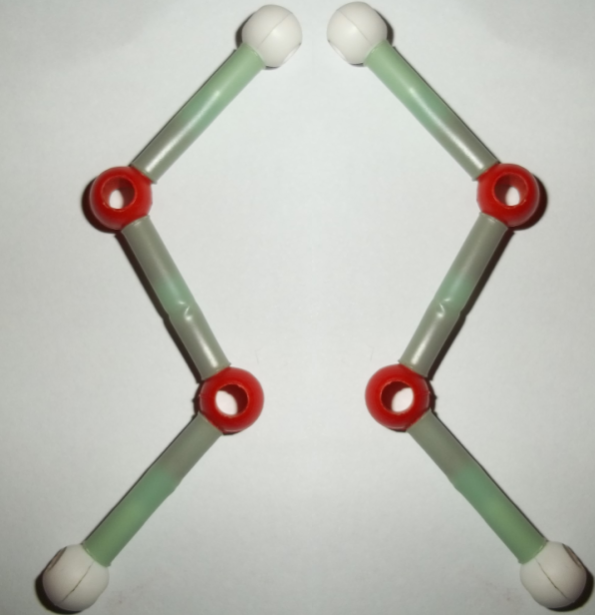
\includegraphics[width=.1\textwidth]{photos/H2O2_models.png} & 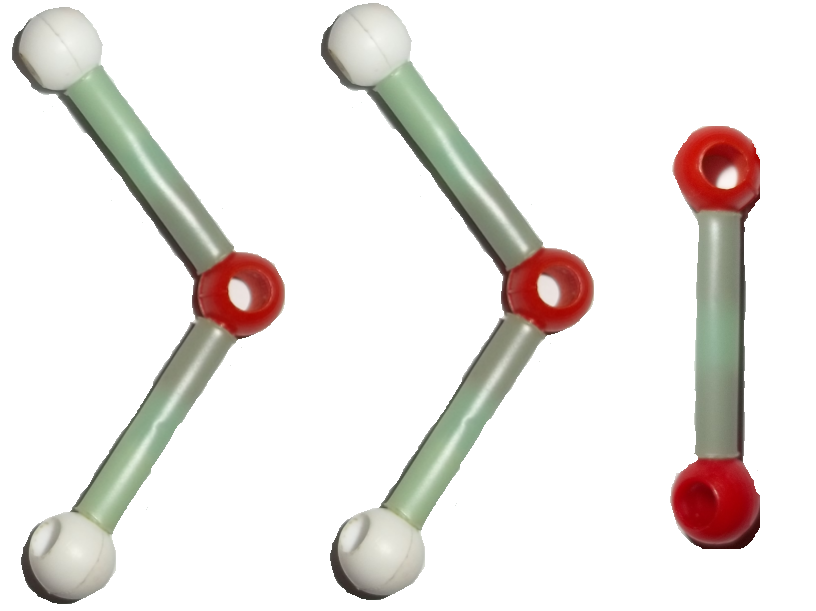
\includegraphics[width=.1\textwidth]{photos/H2O_O2.png} \\ \hline
   \textbf{Molekules} & twee molekules & drie molekules \\ \hline
\textbf{Energie-veranderings} & energie opgeneem wanneer bindings gebreek & energie afgegee wanneer bindings gevorm word \\ \hline
\textbf{Massa konstant} & $4(1,01) + 4(16,0) = 68,04$ & $2(18,02) + 2(16,0) = 68,04$ \\ \hline
\textbf{Atome konstant} & 4 suurstof atome, 4 waterstof atome & 4 suurstof atome, 4 waterstof atome \\ \hline
  \end{tabular}
 \end{center}
\caption{Belangrike begrippe rondom chemiese verandering}
\label{tab:chemchangeconcepts}
\end{table}
\begin{exercises}{Fisiese en chemiese verandering}
{
Vir elkeen van die volgende s\^{e} of 'n chemiese of 'n fisiese verandering plaasvind.
\begin{enumerate}[noitemsep, label=\textbf{\arabic*}. ]
\item Smeltende kerswas.
\item Die meng van natriumchloried ($\text{NaCl}$) en silvernitraat ($\text{AgNO}_3$) om silverchloried ($\text{AgCl}$) te vorm.
\item Die meng van soutsuur ($\text{HCl}$) en magnesiumlint ($\text{Mg}$) om magnesiumchloried ($\text{MgCl}_{2}$) te vorm.
\item Die oplossing van sout in water.
\item Die afskeur van 'n stuk magnesiumlint. 
\end{enumerate}

\insertpracticeinfo{5}
}
\end{exercises}

    \label{m38711*cid5}
            \section{Die behoud van atome en massa in reaksies}
            \nopagebreak
      \label{m38711*id64489}In 'n chemiese reaksie sal die totale massa van al die stowwe wat deelneem aan die reaksie, dieselfde bly. Die aantal  \textbf{atome} in 'n reaksie bly ook dieselfde. Massa kan nie geskep of vernietig word tydens 'n chemiese reaksie nie. \par 

\mindsetvid{conservation of mass}{VPbkj}

\Definition{Die wet van die behoud van massa}{Die wet van die behoud van massa lui dat die totale massa van stowwe wat deelneem aan ‘n chemiese reaksie behoue bly tydens die reaksie.}
Tabel~\ref{tab:chemchangeconcepts} illustreer hierdie wet vir die ontbinding van waterstofperoksied. Die volgende aktiwiteit maak dit vir jou moontlik om dit self te sien met behulp van modelle.
            \begin{activity}{Die behoud van atome in chemiese reaksies}
            \nopagebreak
            \label{m38711*id64844}\noindent
\textbf{Materiale:} \\ Gekleurde klei gerol in balletjies of albasters en “prestick” om atome te verteenwoordig. Elke kleur verteenwoordig 'n ander element.
        \par 
      \label{m38711*id64882}\noindent
\textbf{Metode:}\\
      \label{m38711*id64889}\begin{enumerate}[noitemsep, label=\textbf{\arabic*}. ] 
\label{m38711*uid36}\item Bou you reaktnase. Gebruik albasters en 'prestick' of klei om die reaktanse te verteenwoordig en plaas dit aan die een kant van jou tafel. Maak minstens tien ($\text{H}_{2}$) eenhede en minstens vyf ($\text{O}_{2}$) eenhede.
\label{m38711*uid37}\item Plaas die $\text{H}_{2}$ en $\text{O}_{2}$ eenhede op 'n tafel. Die tafel verteenwoordig die 'proefbuis' waar die reaksie gaan plaasvind.
\label{m38711*uid38}\item Tel nou die aantal atome ($\text{H}$ en $\text{O}$) wat jy in jou 'proefbuis' het. Vul die reaktense-kolom in op die tabel hieronder. Verwys na tabel~\ref{tab:chemchangeconcepts} om jou te help om die massa ry in te vul.
\label{m38711*uid39}\item Laat die reaksie plaasvind. Elke persson kan nou die $\text{H}$ en $\text{O}$ eenhede gebruik om water-eenhede te maak. Breek die $\text{H}$ en $\text{O}$ eenhede uitmekaar en bou $\text{H}_{2}\text{O}$ eenhede met die dele. Dit is die produkte. Plaas die produkte op die tafel. 
\item Wanner die reaksie verby is (dws wanneer al die $\text{H}$ en $\text{O}$ eenhede gebruik is), tel die aantal atome ($\text{H}$ en $\text{O}$) en voltooi die tabel.
\item Wat merk jy op aangaande die getal van die atome vir die reaktanse, in vergelyking met die produkte?
\item Skryf 'n gebalanseerde vergelyking vir hierdie reaksie en gebruik jou modelle om die vergelyking te bou.
\end{enumerate}
        \par 
\begin{table}[H]
 \begin{center}
  \begin{tabular}{|l|l||l|} \hline
& \textbf{Reaktanse} & \textbf{Produkte} \\ 
& 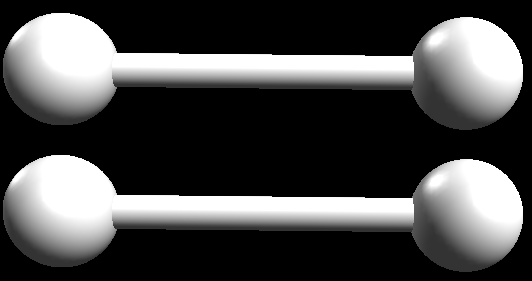
\includegraphics[width=.1\textwidth]{photos/hydrogen.png} 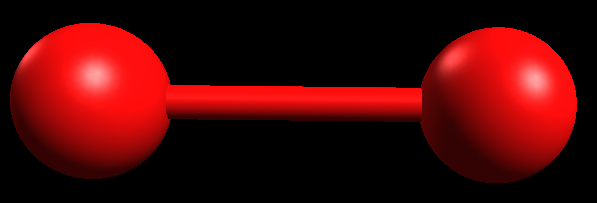
\includegraphics[width=.1\textwidth]{photos/oxygen.png} & \includegraphics[width=.1\textwidth]{photos/water.png} \\ \hline
   \textbf{Aantal molekules} &  &  \\ \hline
\textbf{Massa} &  &  \\ \hline
\textbf{Aantal atome} &  &  \\ \hline
  \end{tabular}

 \end{center}

\end{table}

      \label{m38711*id65031}\noindent{}\textbf{Bespreking}
Jy moes opgemerk het dat die aantal atome in die reaktanse dieselfde is as die aantal atome in die produk. Die aantal atome bly behoue tydens die reaksie. Jy sal egter ook sien dat die molekules in die reaktanse en produkte nie dieselfde is nie. Die aantal molekule bly nie behoue tydens die reaksie nie.
 \par 
\end{activity}
\label{m38711*eip-14}
            \begin{i_experiment}{Behoud van materie}
            \nopagebreak
            \label{m38711*eip-453}\noindent{}\textbf{Doel:}
Die eksperimentele bewys van die wet van die behoud van massa.
\par 
\label{m38711*eip792}\noindent{}\textbf{Materiaal:}
\textsl{Reaksie 1:} \\
3 bekers; lood (II) nitraat; natriumjodied; massameter \\
\textsl{Reaksie 2:} \\
 soutsuur; broomtimolblou; natriumhydroksiedoplossing; massameter \\
 \textsl{Reaksie 3:} \\
enige bruistablet (bv. Cal-C-Vita tablet), ballon; rekkie; massameter; proefbuis; beker
\par 
\label{m38711*eip-153}
\Warning{Wees altyd versigtig wanneer jy chemikalie\"{e} hanteer (veral sterk sure soos soutsuur), want jy kan jouself ernstig verbrand. }
	\par
      \label{m38711*id72432}\noindent
\textbf{Metode:} \\
\begin{minipage}{.6\textwidth}
\textsl{Reaksie 1} 
\label{m38711*id6342}\begin{enumerate}[noitemsep, label=\textbf{\arabic*}. ] 
            \item Oplossing 1: Los $5~\text{g}$ silvernitraat op in $100~\text{ml}$ water.
\item Oplossing 2: Los $4.5~\text{g}$ natriumjodide op in $100~\text{ml}$ water.
\item Bepaal die massa van die reaktanse.
\item Voeg oplossing 1 by oplossing 2. Wat neem jy waar? Het 'n chemiese reaksie plaasgevind? 
\item Bepaal die massa van die produkte. 
\item Wat merk jy op met betrekking tot die massas?
\item Skryf 'n gebalanseerde vergelyking vir hierdie reaksie neer.
\end{enumerate}
\end{minipage}
\begin{minipage}{.4\textwidth}
 \begin{center}
\scalebox{0.6}{
  \begin{pspicture}(0,0)(5,5)
\newpsstyle{white} {linestyle=solid,linewidth=.1,fillstyle=solid,fillcolor=white}
 \pstTubeEssais[etiquette,Numero={ $\text{AgNO}_{2}$},aspectLiquide1=white]
\pstTubeEssais[etiquette,Numero={ $\text{NaI}$},aspectLiquide1=white]  
  \end{pspicture}
}
 \end{center}
\end{minipage}
\begin{minipage}{.6\textwidth}
\textsl{Reaction 2:}
\label{m38711*id63452}\begin{enumerate}[noitemsep, label=\textbf{\arabic*}. ] 
\item Oplossing 1: Los $0.4~\text{g}$ natriumhydroksied op in $100~\text{ml}$ water. Voeg 'n paar druppels broomtimolblou indikator by die oplossing. 
\item Oplossing 2: Meet $100~\text{ml}$ van 'n $0,1~\text{M}$ soutsuuroplossing in 'n beker af. 
\item Bepaal die massa van die reaktanse.
\item Voeg klein hoeveelhede van oplossing 2 by oplossing 1 (jy kan 'n plastiek pipet gebruik hiervoor) totdat 'n kleurverandering plaasgevind het. Het daar 'n chemiese reaksie plaasgevind? 
\item Bepaal die massa van die soutsuur wat bygevoeg is. (Jy doen dit deur die gewig van die oorblywende oplossing af te trek van die oorspronklike massa.)
\item Vergelyk die massa voor die reaksie met die totale massa na die reaksie. Wat neem jy waar?
\item Skryf 'n gebalanseerde vergelyking vir hierdie reaksie neer.
\end{enumerate}
\end{minipage}
\begin{minipage}{.4\textwidth}
 \begin{center}
\scalebox{.7}{
  \begin{pspicture}(0,0)(5,5)
\newpsstyle{white} {linestyle=solid,linewidth=.1,fillstyle=solid,fillcolor=white}
 \pstTubeEssais[etiquette,Numero={ $\text{NaOH}$},aspectLiquide1=white]
\pstTubeEssais[etiquette,Numero={ $\text{HCl}$},aspectLiquide1=white]    
  \end{pspicture}
}
 \end{center}
\end{minipage}
\begin{minipage}{.6\textwidth}
\textbf{Reaksie 3}
\label{m38711*id634223}\begin{enumerate}[noitemsep, label=\textbf{\arabic*}. ] 
\item Vul 'n groot proefbuis halfpad met water.
\item Bepaal die gesamentlike massa van die proefbuis en die water.
\item Breek 'n bruistablet in twee of drie stukkies en plaas dit in 'n ballon.
\item Bepaal die gesamentlike massa van die ballon en die tablet.
\item Pas die ballon styf om die proefbuis; wees versigtig om nie die inhoud in die water te laat val nie. Jy kan die proefbuis binne ‘n beker laat staan om jou te help.
\item Bepaal die totale massa van die proefbuis en ballon.
\item Lig die ballon sodat die tablet in die water beland. Wat neem jy waar? Het 'n chemiese reaksie plaasgevind?
\item Bepaal die massa van die proefbuis-ballon- kombinasie.
\item Wat neem jy waar rakende die massas voor en na afloop van die reaksie?
\end{enumerate}
\end{minipage}
\begin{minipage}{.4\textwidth}
 \begin{center}
\scalebox{.6}{
  \begin{pspicture}(0,0)(5,5)
\newpsstyle{white} {linestyle=solid,linewidth=.1,fillstyle=solid,fillcolor=white}
 \pstTubeEssais[etiquette,Numero={ $\text{H}_{2}\text{O}$},aspectLiquide1=white]
   
  \end{pspicture}
}
 \end{center}
\end{minipage}
        \par \label{m38711*eip-768}\noindent{}\textbf{Resultaat:} Voltooi die volgende tabel vir die totale massa van reaktanse (begin-materiale)
en produkte (einde-materiale).  \par 
    % \textbf{m38711*eip-581}\par
          \begin{table}[H]
    % \begin{table}[H]
    % \\ '' '0'
        \begin{center}
      \label{m38711*eip-581}
      \begin{tabular}{|l|l|l|l|}\hline
         &
        Reaksie 1 &
        Reaksie 2 &
        Reaksie 3 \\ \hline
        Reaktanste &
         &
         &
        \\ \hline
        Produkte &
         &
         &
        \\ \hline
    \end{tabular}
      \end{center}
\end{table}
    \par
  \label{m38711*eip-634}Tel die massas van die reaktanse bymekaar vir elke reaksie. Doen dieselfde vir die produkte. Vergelyk by elke reaksie
die massa van die reaktanse met die massa van die produkte. Wat neem jy waar? Het die massa behoue gebly?
\par \label{m38711*eip-65}In die eksperiment hierbo sal jy vind dat die totale massa aan die begin van die reaksie dieselfde is as aan die einde van
die reaksie. Massa verskyn of verdwyn nie tydens chemiese reaksies nie. Massa bly behoue, met ander woorde, die totale
massa waarmee jy begin sal ooreenstem met die totale massa aan die einde van die reaksie. \par
\end{i_experiment} 

\begin{exercises}{Conservation van atome en massa}
{
Voltooi die volgende chemiese reaksies om aan te toon dat atome en massa behoue bly. Verskaf die totale molekulêre
massa van die reaktanse en die produkte.
 \begin{enumerate}[noitemsep, label=\textbf{\arabic*}.]
  \item Waterstofgas kombineer met stikstofgas om ammoniak te vorm.\\
\begin{figure}[H]
 \begin{center}
\scalebox{.5} % Change this value to rescale the drawing.
{
\begin{pspicture}(0,-2.01)(9.98,2.01)
\psframe[linewidth=0.04,dimen=outer](4.0,2.01)(0.0,-1.99)
\psframe[linewidth=0.04,dimen=outer](9.98,1.99)(5.98,-2.01)
\psline[linewidth=0.07cm,arrowsize=0.05291667cm 3.0,arrowlength=1.4,arrowinset=0.0]{->}(4.58,0.13)(5.42,0.13)
\pscircle[linewidth=0.04,dimen=outer](0.54,1.49){0.16}
\pscircle[linewidth=0.04,dimen=outer](0.84,1.49){0.16}
\rput{-46.441925}(1.196338,1.3458508){\pscircle[linewidth=0.04,dimen=outer](2.1666365,-0.7212986){0.16}}
\rput{-46.441925}(1.4181583,1.428068){\pscircle[linewidth=0.04,dimen=outer](2.3733635,-0.93870145){0.16}}
\rput{31.74865}(0.97520715,-1.4871812){\pscircle[linewidth=0.04,dimen=outer](3.1024454,0.97107095){0.16}}
\rput{31.74865}(1.0964445,-1.597797){\pscircle[linewidth=0.04,dimen=outer](3.3575547,1.1289291){0.16}}
\rput{80.2375}(1.1726402,-4.547286){\pscircle[linewidth=0.04,dimen=outer](3.2845652,-1.5778278){0.16}}
\rput{80.2375}(1.5062582,-4.351896){\pscircle[linewidth=0.04,dimen=outer](3.3354347,-1.2821721){0.16}}
\rput{38.670666}(-0.64319474,-0.8944015){\pscircle[linewidth=0.04,dimen=outer](0.9528874,-1.3637265){0.16}}
\rput{38.670666}(-0.47471237,-0.99965644){\pscircle[linewidth=0.04,dimen=outer](1.1871126,-1.1762736){0.16}}
\pscircle[linewidth=0.04,dimen=outer](0.52,-0.01){0.16}
\pscircle[linewidth=0.04,dimen=outer](0.82,-0.01){0.16}
\pscircle[linewidth=0.04,linecolor=blue,dimen=outer,fillstyle=solid,fillcolor=blue](1.39,0.88){0.25}
\pscircle[linewidth=0.04,linecolor=blue,dimen=outer,fillstyle=solid,fillcolor=blue](1.87,0.86){0.25}
\rput{47.621758}(0.82527715,-2.231293){\pscircle[linewidth=0.04,linecolor=blue,dimen=outer,fillstyle=solid,fillcolor=blue](2.9408476,-0.1805505){0.25}}
\rput{47.621758}(1.1875323,-2.370011){\pscircle[linewidth=0.04,linecolor=blue,dimen=outer,fillstyle=solid,fillcolor=blue](3.2791524,0.1605505){0.25}}
\end{pspicture}
} 
 \end{center}
\end{figure}
\item Waterstofperoksied ontbind (word afgebreek) om waterstof en suurstof te vorm.\\
\begin{figure}[H]
 \begin{center}
\scalebox{.5} % Change this value to rescale the drawing.
{
\begin{pspicture}(0,-2.01)(9.98,2.01)
\psframe[linewidth=0.04,dimen=outer](4.0,2.01)(0.0,-1.99)
\psframe[linewidth=0.04,dimen=outer](9.98,1.99)(5.98,-2.01)
\psline[linewidth=0.07cm,arrowsize=0.05291667cm 3.0,arrowlength=1.4,arrowinset=0.0]{->}(4.58,0.13)(5.42,0.13)
\pscircle[linewidth=0.04,dimen=outer](0.62,1.39){0.16}
\pscircle[linewidth=0.04,linecolor=red,dimen=outer,fillstyle=solid,fillcolor=red](0.83,1.04){0.25}
\pscircle[linewidth=0.04,dimen=outer](1.54,0.69){0.16}
\pscircle[linewidth=0.04,linecolor=red,dimen=outer,fillstyle=solid,fillcolor=red](1.31,1.02){0.25}
\rput{-39.021122}(0.33611158,0.5916722){\pscircle[linewidth=0.04,dimen=outer](1.002982,-0.17846099){0.16}}
\rput{-39.021122}(0.57779634,0.46549466){\pscircle[linewidth=0.04,linecolor=red,dimen=outer,fillstyle=solid,fillcolor=red](0.9457715,-0.58259827){0.25}}
\rput{-39.021122}(1.1043428,0.513664){\pscircle[linewidth=0.04,dimen=outer](1.277018,-1.3015391){0.16}}
\rput{-39.021122}(0.8582375,0.6214732){\pscircle[linewidth=0.04,linecolor=red,dimen=outer,fillstyle=solid,fillcolor=red](1.3060981,-0.9003478){0.25}}
\rput{-93.27925}(2.4115129,4.595749){\pscircle[linewidth=0.04,dimen=outer](3.37574,1.159226){0.16}}
\rput{-93.27925}(2.218723,4.0344186){\pscircle[linewidth=0.04,linecolor=red,dimen=outer,fillstyle=solid,fillcolor=red](3.0143006,0.96959066){0.25}}
\rput{-93.27925}(2.4940598,2.916798){\pscircle[linewidth=0.04,dimen=outer](2.62426,0.28077406){0.16}}
\rput{-93.27925}(2.645873,3.4816551){\pscircle[linewidth=0.04,linecolor=red,dimen=outer,fillstyle=solid,fillcolor=red](2.9668763,0.49152064){0.25}}
\rput{62.03058}(0.100764476,-3.0118408){\pscircle[linewidth=0.04,dimen=outer](2.5551405,-1.4221209){0.16}}
\rput{62.03058}(0.33603603,-3.360519){\pscircle[linewidth=0.04,linecolor=red,dimen=outer,fillstyle=solid,fillcolor=red](2.96275,-1.4007995){0.25}}
\rput{62.03058}(1.0858464,-3.6818182){\pscircle[linewidth=0.04,dimen=outer](3.6048594,-0.937879){0.16}}
\rput{62.03058}(0.8310885,-3.354817){\pscircle[linewidth=0.04,linecolor=red,dimen=outer,fillstyle=solid,fillcolor=red](3.205534,-0.98624444){0.25}}
\end{pspicture} 
}
 \end{center}
\end{figure}
\item Kalsium en suurstofgas reageer om kalsiumoksied te vorm.\\
\begin{figure}[H]
 \begin{center}
\scalebox{.5} % Change this value to rescale the drawing.
{
\begin{pspicture}(0,-2.01)(9.98,2.01)
\definecolor{color314b}{rgb}{0.5019607843137255,0.0,1.0}
\psframe[linewidth=0.04,dimen=outer](4.0,2.01)(0.0,-1.99)
\psframe[linewidth=0.04,dimen=outer](9.98,1.99)(5.98,-2.01)
\psline[linewidth=0.07cm,arrowsize=0.05291667cm 3.0,arrowlength=1.4,arrowinset=0.0]{->}(4.58,0.13)(5.42,0.13)
\pscircle[linewidth=0.04,dimen=outer](0.54,1.49){0.16}
\pscircle[linewidth=0.04,dimen=outer](0.84,1.49){0.16}
\rput{38.670666}(0.8036014,-1.5376498){\pscircle[linewidth=0.04,dimen=outer](2.5928874,0.37627354){0.16}}
\rput{38.670666}(0.97208375,-1.6429048){\pscircle[linewidth=0.04,dimen=outer](2.8271127,0.5637264){0.16}}
\rput{112.262375}(0.40818247,-2.4516025){\pscircle[linewidth=0.04,dimen=outer](1.0268273,-1.0888188){0.16}}
\rput{112.262375}(0.5084122,-1.9635997){\pscircle[linewidth=0.04,dimen=outer](0.9131727,-0.8111812){0.16}}
\pscircle[linewidth=0.04,linecolor=color314b,dimen=outer,fillstyle=solid,fillcolor=color314b](1.61,1.16){0.25}
\pscircle[linewidth=0.04,linecolor=color314b,dimen=outer,fillstyle=solid,fillcolor=color314b](1.91,-0.26){0.25}
\pscircle[linewidth=0.04,linecolor=color314b,dimen=outer,fillstyle=solid,fillcolor=color314b](3.35,1.3){0.25}
\pscircle[linewidth=0.04,linecolor=color314b,dimen=outer,fillstyle=solid,fillcolor=color314b](0.49,0.06){0.25}
\pscircle[linewidth=0.04,linecolor=color314b,dimen=outer,fillstyle=solid,fillcolor=color314b](2.05,-1.42){0.25}
\pscircle[linewidth=0.04,linecolor=color314b,dimen=outer,fillstyle=solid,fillcolor=color314b](3.33,-0.94){0.25}
\end{pspicture} 
}
 \end{center}
\end{figure}
 \end{enumerate}

\insertpracticeinfo{3}
}
\end{exercises}

    \label{m38711*cid6}
            \section{Die wet van konstante samestelling}
            \nopagebreak
      \label{m38711*id65065}In enige gegewe chemiese verbinding kombineer die elemente altyd in dieselfde verhouding met mekaar. Die is \textbf{die wet van konstante verhouding}.\par 
\label{m38711*id65075}Die \textbf{wet van konstante samestelling} s\^{e} dat, in 'n spesifieke chemiese verbinding, al die voorbeelde
van die verbinding gemaak sal word van dieselfde elemente in dieselfde verhouding. Byvoorbeeld, enige watermolekule is
altyd saamgestel uit twee waterstofatome en een suurstofatoom in 'n 2:1 verhouding. As ons kyk na die relatiewe massas van suurstof en waterstof in 'n watermolekuul, sal ons sien dat 94\% van die massa van 'n watermolekuul bygedra word deur suurstof en die oorblywende 6\% is afkonstig van die massa van waterstof. Hierdie massa-verhouding sal dieselfde wees vir enige water molekule.\par 
      \label{m38711*id65089}Dit beteken nie dat waterstof en suurstof altyd kombineer in 'n 2:! verhouding om $\text{H}{}_{2}\text{O}$. Verskillende verhoudings is moontlik. Byvoorbeeld, watersof en suurstof kombineer in verskillende verhoudings om $\text{H}{}_{2}\text{O}{}_{2}$ te vorm eerder as $\text{H}{}_{2}\text{O}$. In $\text{H}{}_{2}\text{O}{}_{2}$, is die H:O verhouding 1:1 en die massa verhouding van waterstof tot suurstof 1:16. Dit sal dieselfde wees vir enige molekule van waterstofperoksied.\par 
\begin{Investigation}{Die wet van konstante samestelling}
 \textbf{Doel:} \\
Om ondersoek in te stel na die verhouding waarin verbindings kombineer. \\
\textbf{Apparatus:} \\
\begin{minipage}{.4\textwidth}
\begin{itemize}[noitemsep]
\item $0,1~\text{M}$ silvernitraat ($\text{AgNO}_3$)
\item $0,1~\text{M}$ natriumchloried ($\text{NaCl}$)
\item $0,1~\text{M}$ loodnitraat ($\text{PbNO}_{3}$)
\item $0,1~\text{M}$ natriumjodide ($\text{NaI}$)
\item $0,1~\text{M}$ yster (III) chloried ($\text{FeCl}_{3}$)
\item $0,1~\text{M}$ natriumhydroksied ($\text{NaOH}$)
\item 9 proefbuise
\item 3 propette
\end{itemize}
\end{minipage} 
\begin{minipage}{.6\textwidth}
 \begin{center}
\scalebox{.7}{
  \begin{pspicture}(0,0)(6,6)
\psset{unit=.5}
\newpsstyle{white} {linestyle=solid,linewidth=.1,fillstyle=solid,fillcolor=white}
\newpsstyle{orange} {linestyle=solid,linewidth=.1,fillstyle=solid,fillcolor=white!20!orange}
%Silver nitrate
 \pstTubeEssais[etiquette,Numero={ $\text{AgNO}_3$},aspectLiquide1=white,niveauLiquide1=10]
\pstTubeEssais[etiquette,Numero={ $\text{AgNO}_3$},aspectLiquide1=white,niveauLiquide1=15] 
 \pstTubeEssais[etiquette,Numero={ $\text{AgNO}_3$},aspectLiquide1=white,niveauLiquide1=20]
%Lead nitrate
\pstTubeEssais[etiquette,Numero={$\text{PbNO}_{3}$},aspectLiquide1=white,niveauLiquide1=10]  
 \pstTubeEssais[etiquette,Numero={$\text{PbNO}_{3}$},aspectLiquide1=white,niveauLiquide1=15]
\pstTubeEssais[etiquette,Numero={$\text{PbNO}_{3}$},aspectLiquide1=white,niveauLiquide1=20]
% Iron (III) chloride
 \pstTubeEssais[etiquette,Numero={$\text{FeCl}_{3}$},aspectLiquide1=orange,niveauLiquide1=10]
\pstTubeEssais[etiquette,Numero={$\text{FeCl}_{3}$},aspectLiquide1=orange,niveauLiquide1=15]  
 \pstTubeEssais[etiquette,Numero={$\text{FeCl}_{3}$},aspectLiquide1=orange,niveauLiquide1=20] 
  \end{pspicture}
}
 \end{center}
\end{minipage}
\textbf{Method:}\\
\textsl{Reaksie 1:} Berei drie proefbuise met $5~\text{ml}$, $10~\text{ml}$ en $15~\text{ml}$ van silvernitraat onderskeidelik. Met behulp van 'n skoon propette voeg $5~\text{ml}$ van natriumchloried aan elkeen en sien wat gebeur. Skryf 'n gebalanseerde vergelyking vir hierdie reaksie.\\
\textsl{Reaksie 2:} Berei drie proefbuise met $5~\text{ml}$, $10~\text{ml}$ en $15~\text{ml}$  van loodnitraat onderskeidelik. Met behulp van 'n skoon propette voeg $5~\text{ml}$ van natriumjodide aan elkeen en sien wat gebeur. Skryf 'n gebalanseerde vergelyking vir hierdie reaksie.\\
\textsl{Reaksie 3:} Berei drie proefbuise met $5~\text{ml}$, $10~\text{ml}$ en $15~\text{ml}$  van natriumhydroksied onderskeidelik. Voeg $5~\text{ml}$ van iron(III) chloried aan elkeen en sien wat gebeur. Skryf 'n gebalanseerde vergelyking vir hierdie reaksie. \\
\textbf{Bespreking en gevolgtrekking:} \\
By elkeen van die drie voorbeelde sou jy gevind het dat 'n reaksie plaasvind (soos gesien kan word aan die teenwoordigheid van 'n neerslag) sodra die hoeveelheid van die reaktanse groter of gelyk is aan die verhouding waarin die reaktanse kombineer.  
\end{Investigation}

    \label{m38711*cid7}
            \subsection*{Volume verhoudings in gasse}
            \nopagebreak
      \label{m38711*id65179}In 'n chemiese reaksie tussen gasse is die relatiewe volumes van die gasse in die reaksie aanwesig in 'n verhouding van klein heelgetalle indien al die gasse by dieselfde temperatuur en druk verkeer. Hierdie verhouding staan ook bekend as \textbf{Gay-Lussac se Wet}.\par 
      \label{m38711*id65189}Byvoorbeeld, in die reaksie tussen waterstof en suurstof om water te vorm, sal twee volumes $\text{H}{}_{2}$ reageer met 1 volume van $\text{O}_{2}$ om 2 volumes van $\text{H}_{2}\text{O}$ te produseer.\par 
      \label{m38711*id65237}$2\text{H}_{2}\text{g} +\text{O}_{2} \text{(g)} \to 2\text{H}_{2}\text{O} (\ell)$\par 
      \label{m38711*id65282}In die reaksie om ammoniak te produseer, sal een volume van stikstofgas reageer met drie volumes waterstofgas om twee volumes ammoniakgas te produeer.\par 
      \label{m38711*id65286}$\text{N}_{2} \text{(g)}+3\text{H}_{2} \text{(g)} \to 2\text{NH}_{3} \text{(g)}$
      \par  
    \label{m38711*cid8}

\summary{VPdwh}
            \nopagebreak
% \label{m38711*id972312}
% Die volgende video verskaf 'n opsomming van die begrippe wat in hierdie hoofstuk gedek word.
%     \setcounter{subfigure}{0}
% 	\begin{figure}[H] % horizontal\label{m38711*summary}
%     \textnormal{Physical and chemical change}\vspace{.1in} \nopagebreak
%   \label{m38711*yt-media1}\label{m38711*yt-video1}
%             \raisebox{-5 pt}{ 
\includegraphics[width=0.5cm]{col11305.imgs/summary_www.png}} { (Video:  P10058 )}
%  \end{figure}       
% \par  \vspace{-1cm}
      \label{m38711*id65342}\begin{enumerate}[noitemsep, label=\textbf{\arabic*}. ] 
            \label{m38711*uid40}\item Materie bly nie dieselfde nie. Dit kan fisiese of chemiese veranderinge ondergaan.
\label{m38711*uid41}\item 'n \textbf{Fisiese verandering} beteken dat die vorm van materie kan verandr, maar nie sy identiteit nie. Byvoorbeeld, wanner water verdamp sal die energie en die rangskikking van watermolekules verander, maar die struktuur van die water molekules self nie.
\label{m38711*uid42}\item Tydens 'n fisiese verandering, kan die \textbf{rangskikking van deeltjies} verander, maar die massa, aantal atome en die aantal molekules sal dieselfde bly.
\label{m38711*uid43}\item Fisiese veranderings behels klein veranderings in \textbf{energie} en is maklik onkeerbaar.
\label{m38711*uid44}\item 'n Chemiese verandering vind plaas wanneer een of meer stowwe verander na ‘n ander materiaal. 'n
Chemiese reaksie behels die vorming van nuwe produkte met \textbf{verskillende eienskappe}. Byvoorbeeld, magnesium en suurstof reageer om magnesiumoksied ($\text{MgO}$) te vorm.
\label{m38711*uid45}\item 'n Chemiese verandering kan 'n \textbf{ontbinding} of \textbf{syntese} reaksie behels. Tydens chemiese
verandering sal die massa en aantal atome dieselfde bly, maar die aantal molekules bly nie altyd dieselfde nie.
\label{m38711*uid46}\item Chemiese reaksies behels groot veranderinge in energie. Chemiese reaksies is nie maklik omkeerbaar nie.
\label{m38711*uid48}\item Die \textbf{wet van die behoud van massa} stel dat die totale massa van al die stowwe wat deelneem aan 'n chemiese reaksie behoue bly en dat die aantal atome van elke element in die reaksie nie verander wanneer 'n nuwe produk gevorm word nie.
\label{m38711*uid49}\item Die \textbf{bewaring van energie beginsel} stel dat energie nie geskep of vernietig kan word nie, maar net kan verander van een vorm na 'n ander.
\label{m38711*uid50}\item Die \textbf{wet van konstante samestelling} behels dat vir enige bepaalde verbinding, al die voorbeelde van daardie verbinding gemaak sal word van dieselfde elemente in dieselfde verhouding.
\label{m38711*uid51}\item \textbf{Gay-Lussac se wet} bepaal dat in 'n chemiese reaksie tussen gasse, die relatiewe volumes van die gasse in die reaksie teenwoordig is in 'n verhouding van klein heelgetalle indien al die gasse by dieselfde temperatuur en druk verkeer.
\end{enumerate}
\label{m38711*secfhsst!!!underscore!!!id584}
            \begin{eocexercises}{Fisiese en chemiese verandering}
            \nopagebreak
      \label{m38711*id65631}\begin{enumerate}[noitemsep, label=\textbf{\arabic*}. ] 
            \label{m38711*uid6234}\item Gee een word of term vir elk van die volgende definisies:
\label{m38711*id632243}\begin{enumerate}[noitemsep, label=\textbf{\alph*}. ] 
            \item 'n Verandering wat waargeneem of gevoel kan word , waar die deeltjies wat betrokke is nie op enige wyse afgebreek word nie
\item Die vorming van nuwe stowwe tydens 'n chemiese reaksie
\item 'n Reaksie waar 'n nuwe produk gevorm word uit elemente of kleiner verbindings \end{enumerate}
\label{m38711*id63272}\item Noem die behoud van energie beginsel.\newline
\label{m38711*id6244}\item Verduidelik hoe 'n chemiese verandering verskil van 'n fisiese verandering.\newline
\label{m38711*uid52}\item Voltooi die volgende tabel deur te sê of elkeen van die beskrywings 'n voorbeeld van 'n fisiese of chemiese verandering is:
    % \textbf{m38711*id65648}\par
          \begin{table}[H]
    % \begin{table}[H]
    % \\ 'id2931526' '1'
        \begin{center}
      \label{m38711*id65648}
    \noindent
      \begin{tabular}{|l|l|}\hline
        \textbf{Beskrywing} &
        \textbf{Fisies of chemies} \\ \hline
        warm en kou water meng &
     \\ \hline
        melk word suur &
     \\ \hline
        'n motor begin roes &
       \\ \hline
        voedsel verteer in die maag &
       \\ \hline
        alkohol verdwyn wanneer dit geplaas word op jou vel &
       \\ \hline
       verhitting van voedsel in 'n mikrogolfoond &
     \\ \hline
        skeiding van sand en gruis &
       \\ \hline
        vuurwerke ontplof &
       \\ \hline
    \end{tabular}
      \end{center}
\end{table}
    \par
          \label{m38711*uid53}\item Vir elk van die volgende reaksies, s\^{e} of dit 'n voorbeeld is van 'n sintese of ontbindingsreaksie:
\label{m38711*id65862}\begin{enumerate}[noitemsep, label=\textbf{\alph*}. ] 
            \label{m38711*uid54}\item 
$\left({\text{NH}}_{4}{\right)}_{2}{\text{CO}}_{3}\to {\text{NH}}_{3}+{\text{CO}}_{2}+\text{H}{}_{2}\text{O}$
\label{m38711*uid56}\item ${\text{N}}_{2}\left(\text{g}\right)+3{\text{H}}_{2}\left(\text{g}\right)\to 2{\text{NH}}_{3}$\label{m38711*uid57}\item 
${\text{CaCO}}_{3}\left(\text{s}\right)\to \text{CaO}+{\text{CO}}_{2}$\end{enumerate}
                \label{m38711*uid58}\item Vir die volgende vergelyking:
${\text{CaCO}}_{3}\left(\text{s}\right)\to \text{CaO}+{\text{CO}}_{2}$
toon aan dat die wet van die behoud van massa geld. Teken sub-mikrospokiese diagramme om die reaksie te verteenwoordig.\newline
        \end{enumerate}

\practiceinfo
\begin{tabular}[h]{cccccc}
 (1.) l2z  &  (2.) l2u  &  (3.) l2J  &  (4.) l3q  &  (5.) l3l  &  (6.) l3i  &
\end{tabular}
\end{eocexercises}
